\section{Robustness}

\begin{figure}%
	\centering
	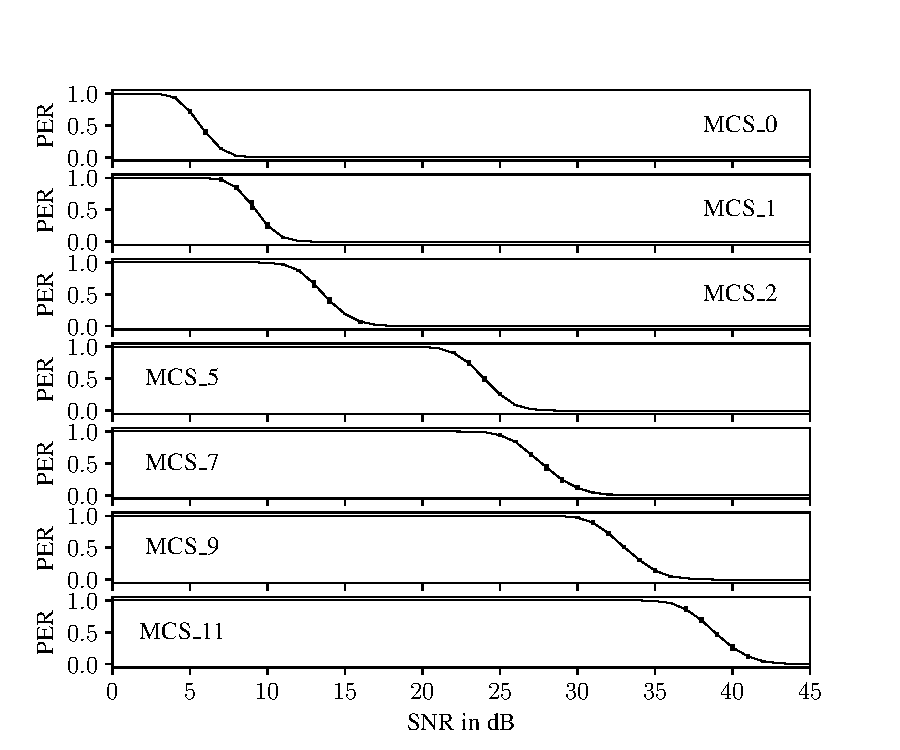
\includegraphics[width=0.95\textwidth]{figures/MCS_PER_to_SNR.pdf}
	\caption{Achieved Goodput and theoretical Datarate of two WiFi 6 stations in Ad-Hoc Mode with a \ac{GI} of \SI{3200}{\nano\second} and a bandwidth of \SI{40}{\mega\hertz} in regards to the number of the chosen \ac{MCS} and \ac{CR} and whether \ac{DCM} is enabled}%
	\label{fig:PER_SNR_MCS}%
\end{figure}


\begin{figure}%
	\centering
	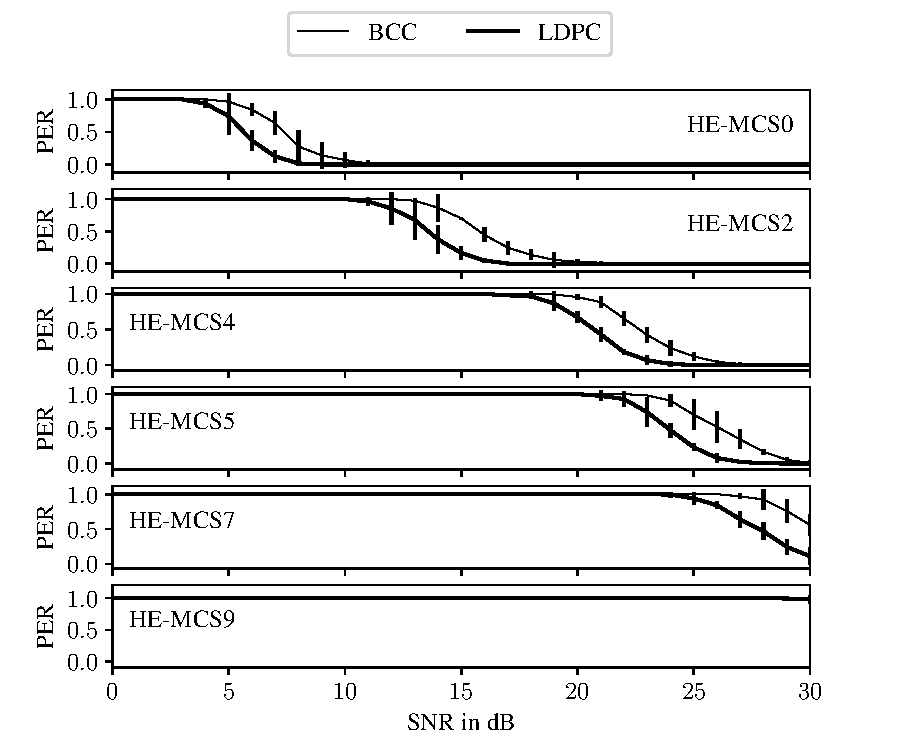
\includegraphics[width=0.95\textwidth]{figures/LDPC_PER_to_SNR.pdf}
	\caption{Simulated \ac{PER} in regards to \ac{SNR} for chosen HE-\ac{MCS} values and whether \ac{LDPC} or \ac{BCC} is enabled for IEEE 802.11ax physical layer parameters of a \ac{GI} of \SI{3200}{\nano\second}, a bandwidth of \SI{20}{\mega\hertz} and 2 spatial streams}%
	\label{fig:PER_SNR_LDPC}%
\end{figure}

\begin{figure}%
	\centering
	
\includegraphics[width=0.95\textwidth]{figures/GI_PER_to_SNR.pdf}
	\caption{Achieved Goodput and theoretical Datarate of two WiFi 6 stations in Ad-Hoc Mode with a \ac{GI} of \SI{3200}{\nano\second} and a bandwidth of \SI{40}{\mega\hertz} in regards to the number of the chosen \ac{MCS} and \ac{CR} and whether \ac{DCM} is enabled}%
	\label{fig:PER_SNR_GI}%
\end{figure}

\begin{figure}%
	\centering
	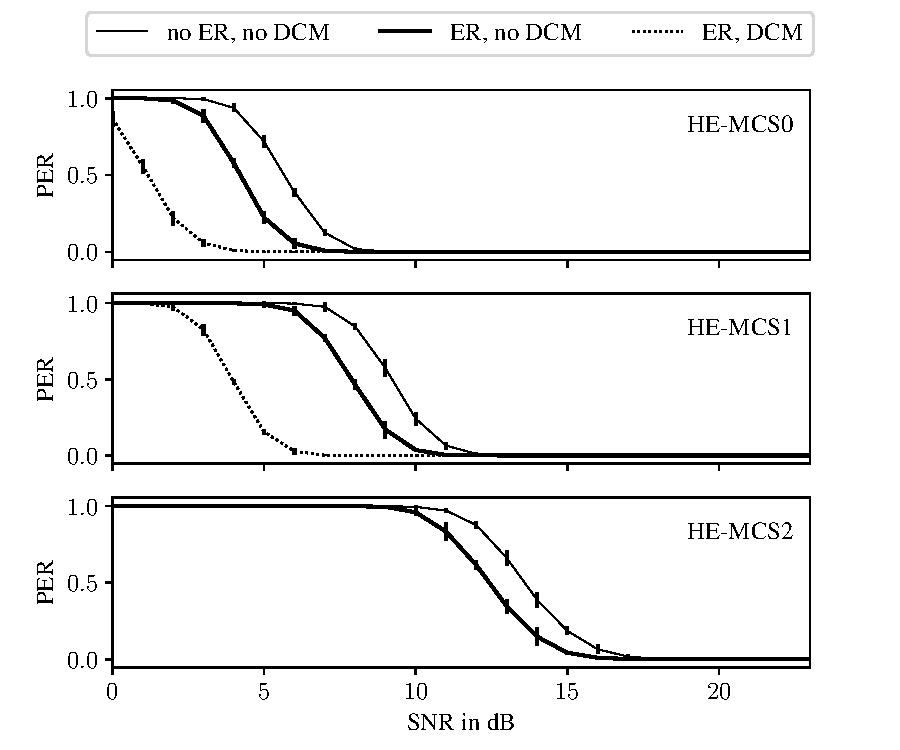
\includegraphics[width=0.95\textwidth]{figures/ER_PER_to_SNR.pdf}
	\caption{Simulated \ac{PER} in regards to \ac{SNR} for chosen HE-\ac{MCS} values and whether Extended Range or \ac{DCM}
	is enabled for IEEE 802.11ax physical layer parameters of a \ac{GI} of \SI{3200}{\nano\second}, a \ac{BW} of \SI{20}{\mega\hertz} and 2 spatial streams}
	\label{fig:PER_SNR_ER}%
\end{figure}

\begin{figure}%
	\centering
	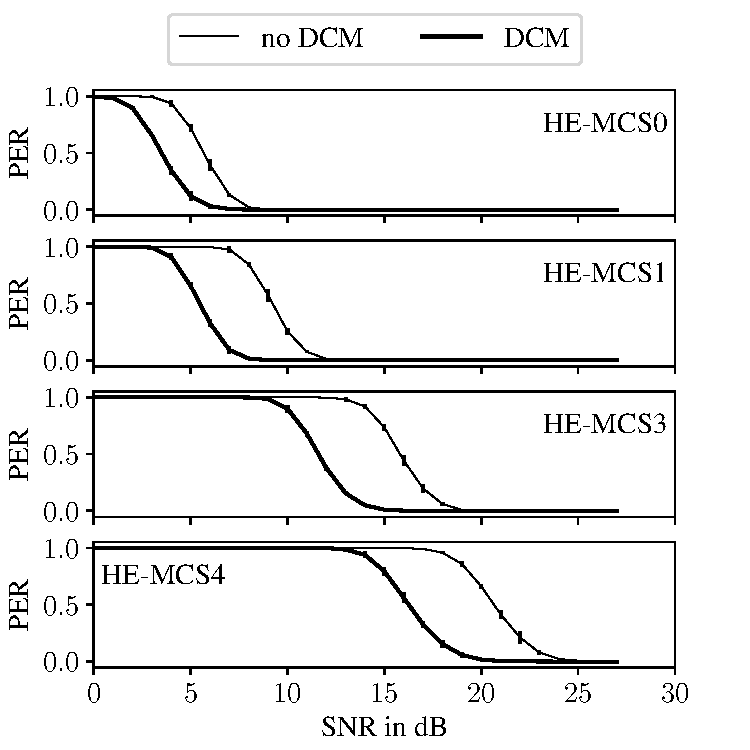
\includegraphics[width=0.95\textwidth]{figures/DCM_PER_to_SNR.pdf}
	\caption{Simulated \ac{PER} in regards to \ac{SNR} for chosen HE-\ac{MCS} values and whether \ac{DCM} is enabled for IEEE 802.11ax physical layer parameters of a \ac{GI} of \SI{3200}{\nano\second}, a \ac{BW} of \SI{20}{\mega\hertz} and 2 spatial streams}%
	\label{fig:PER_SNR_DCM}%
\end{figure}

\begin{figure}%
	\centering
	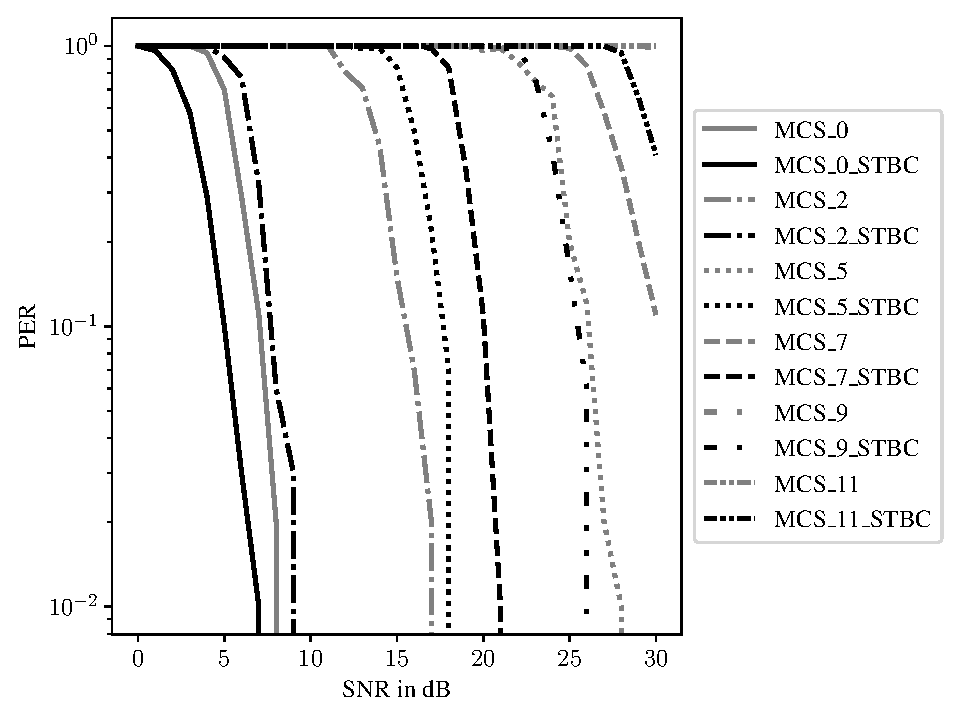
\includegraphics[width=0.95\textwidth]{figures/STBC_PER_to_SNR.pdf}
	\caption{Simulated \ac{PER} in regards to \ac{SNR} for chosen HE-\ac{MCS} values and whether \ac{STBC} is enabled for IEEE 802.11ax physical layer parameters of a \ac{GI} of \SI{3200}{\nano\second}, a \ac{BW} of \SI{20}{\mega\hertz} and 2 spatial streams}%
	\label{fig:PER_SNR_STBC}%
\end{figure}